% Generated by final/appendix/generate.py; edit sources.json.

\FinalAppendixDivider{A}{Architecture and Implementation}{architecture}{Voxelization, reusable blocks, encoder code, spatial alignment, attention, fusion, and decoding.}
\FinalWeeklyAppendixPage{7}{LiDAR Preprocessing}
\FinalWeeklyAppendixPage{8}{Voxelization}
\FinalWeeklyAppendixPage{10}{Normalization and Activation}
\FinalWeeklyAppendixPage{11}{2D Unit}
\FinalWeeklyAppendixPage{12}{2D Unit: Variants}
\FinalWeeklyAppendixPage{13}{2D Pointwise Unit}
\FinalWeeklyAppendixPage{14}{Decoder Block}
\FinalWeeklyAppendixPage{15}{3D Convolution}
\FinalWeeklyAppendixPage{16}{Encoder Stage}
\FinalWeeklyAppendixPage{17}{Upsample and Concat}
\FinalWeeklyAppendixPage{18}{Decoder Stage}
\FinalWeeklyAppendixPage{20}{Encoder Pipeline}
\FinalWeeklyAppendixPage{21}{Encoder Code}
\FinalWeeklyAppendixPage{23}{DiscoGraph}
\FinalWeeklyAppendixPage{24}{DiscoGraph: Feature Alignment}
\FinalWeeklyAppendixPage{25}{DiscoGraph: Rotate and Translate}
\FinalWeeklyAppendixPage{26}{DiscoGraph: Alignment in PyTorch}
\FinalWeeklyAppendixPage{27}{DiscoGraph: Pair the Features}
\FinalWeeklyAppendixPage{28}{DiscoGraph: Edge Scores}
\FinalWeeklyAppendixPage{29}{DiscoGraph: Spatial Weights}
\FinalWeeklyAppendixPage{30}{DiscoGraph: Weighted Features}
\FinalWeeklyAppendixPage{31}{DiscoGraph: Fused Features}
\FinalWeeklyAppendixPage{33}{Decoder Pipeline}

\FinalAppendixDivider{B}{Evaluation and Reproduction}{evaluation}{IoU, confidence scores, precision and recall, AP, dataset statistics, camera views, and benchmark results.}
\FinalWeeklyAppendixPage{35}{Intersection over Union (IoU)}
\FinalWeeklyAppendixPage{36}{IoU: Matching Thresholds}
\FinalWeeklyAppendixPage{37}{DiscoNet Confidence Scores}
\FinalWeeklyAppendixPage{38}{Precision, Recall, and AP}
\FinalWeeklyAppendixPage{39}{V2X-Sim 2.0: Dataset Analysis}
\FinalWeeklyAppendixPage{40}{V2X-Sim 2.0: Car Detections}
\FinalWeeklyAppendixPage{41}{V2X-Sim 2.0: Camera Views}
\FinalWeeklyAppendixPage{42}{Experiment Setup}
\FinalWeeklyAppendixPage{43}{V2X-Sim 2.0: Reproduced Results}
\FinalWeeklyAppendixPage{44}{V2X-Sim 2.0: Runtime Scaling}

\FinalAppendixDivider{C}{Conv2D and Conv3D}{convolutions}{The complete numerical walkthrough: input tensor, kernels, and every spatial and temporal sliding window.}
\FinalWeeklyAppendixPage{50}{Initial Tensor}
\FinalWeeklyAppendixPage{51}{Kernels}
\FinalWeeklyAppendixPage{52}{Conv2D: Sliding Window}
\FinalWeeklyAppendixPage{53}{Conv2D: Sliding Window}
\FinalWeeklyAppendixPage{54}{Conv2D: Sliding Window}
\FinalWeeklyAppendixPage{55}{Conv2D: Sliding Window}
\FinalWeeklyAppendixPage{56}{Conv2D: Sliding Window}
\FinalWeeklyAppendixPage{57}{Conv2D: Sliding Window}
\FinalWeeklyAppendixPage{58}{Conv3D: Sliding Window}
\FinalWeeklyAppendixPage{59}{Conv3D: Sliding Window}
\FinalWeeklyAppendixPage{60}{Conv3D: Sliding Window}
\FinalWeeklyAppendixPage{61}{Conv3D: Sliding Window}
\FinalWeeklyAppendixPage{62}{Conv3D: Sliding Window}
\FinalWeeklyAppendixPage{63}{Conv3D: Sliding Window}
\FinalWeeklyAppendixPage{64}{Conv3D: Sliding Window}
\FinalWeeklyAppendixPage{65}{Conv3D: Sliding Window}
\FinalWeeklyAppendixPage{66}{Conv3D: Sliding Window}
\FinalWeeklyAppendixPage{67}{Conv3D: Sliding Window}
\FinalWeeklyAppendixPage{68}{Conv3D: Sliding Window}
\FinalWeeklyAppendixPage{69}{Conv3D: Sliding Window}

\FinalAppendixDivider{D}{Complete Experiment Record}{experiments}{All 20 report pages: recorded examples, training and test protocol, losses, runtime scaling, and Original/Tree results.}
\FinalExperimentAppendixPage{1}{DiscoNet: Our First Experiment}
\FinalExperimentAppendixPage{2}{Example 1: Reference and Predicted Car Boxes}
\FinalExperimentAppendixPage{3}{Example 1: Camera Views}
\FinalExperimentAppendixPage{4}{V2X-Sim 2.0: Dataset Overview}
\FinalExperimentAppendixPage{5}{Authors' Training Setup and Dataset Splits}
\FinalExperimentAppendixPage{6}{Dataset Statistics by Partition and Vehicle Inputs}
\FinalExperimentAppendixPage{7}{Experiment Setup: Hardware and Software}
\FinalExperimentAppendixPage{8}{Experiment Procedure, Metrics, and Running Time}
\FinalExperimentAppendixPage{9}{Original Test Split: Loss and Detection Accuracy}
\FinalExperimentAppendixPage{10}{How DiscoNet Computes Confidence Scores}
\FinalExperimentAppendixPage{11}{How Precision–Recall Curves and AP Are Computed}
\FinalExperimentAppendixPage{12}{Original Test Split: Accuracy and Loss Plots}
\FinalExperimentAppendixPage{13}{Custom Experiments}
\FinalExperimentAppendixPage{14}{Custom Experiment 1: V2X-Sim Inputs and Replay}
\FinalExperimentAppendixPage{15}{Custom Experiment 1: Measuring Runtime}
\FinalExperimentAppendixPage{16}{Custom Experiment 1: Runtime Results for n = 1–10}
\FinalExperimentAppendixPage{17}{Custom Experiment 1: Runtime Results for n = 11–20}
\FinalExperimentAppendixPage{18}{Custom Experiment 1: Runtime Versus Model Input Count}
\FinalExperimentAppendixPage{19}{Custom Experiment 2: Coarse Attention and Kruskal Fusion}
\FinalExperimentAppendixPage{20}{Custom Experiment 2: Runtime and Detection AP}

\FinalAppendixDivider{E}{Image Generation Example}{image-generation}{Codex CLI, the generation prompt, and the result.}
\begin{frame}{Simple Workflow}
  \SlideBody{%
    {\fontsize{13}{17}\selectfont
    \textbf{I used OpenAI Codex CLI with my ChatGPT account.}\par}
    \vspace{0.40cm}
    {\fontsize{12}{16}\selectfont
    \textbf{Get Access:} Use a
    \href{https://learn.chatgpt.com/docs/pricing}{ChatGPT Plus or Pro subscription},
    install \href{https://learn.chatgpt.com/docs/codex/cli}{Codex CLI},
    and choose \textbf{Sign in with ChatGPT}.\par
    \vspace{0.45cm}
    \textbf{1.} Describe the image in a prompt.\par
    \vspace{0.22cm}
    \textbf{2.} Put the generated image in the slide.\par}
  }
  \SlideSource{OpenAI documentation:
    \href{https://learn.chatgpt.com/docs/codex/cli}{Codex CLI} and
    \href{https://learn.chatgpt.com/docs/pricing}{ChatGPT subscriptions}.}
\end{frame}

\begin{frame}{Prompt: Generate the Image}
  \SlideBody{%
    \vspace{0.12cm}
    {\fontsize{10.5}{13.2}\selectfont
    Can u make a clear image with image-gen for the cooperative perception slide? I'd like three views side by side of the same scene, like a clean 3D illustration seen diagonally from above, on a white background. Car A is behind a big gray truck, and a smaller gray car is in front of that truck, hidden from A. Car B is in the next lane and can see around the truck. Give A a cyan color and B an orange one, with a little LiDAR on each roof. In the first view show only A's cyan points, in the second B's orange points reaching the small car, and in the last put the two together. Keep all four vehicles in the same positions in every view; the small car is just faint gray context in the first, with no cyan points on it. Put a plus and an arrow between the views. No slide title, trees, buildings or extra text, just A and B.
\par}
  }
  \SlideSource{Tested reconstruction; November 9, 2026.}
\end{frame}

\begin{frame}{Generated Result}
  \SlideBody{\centering
    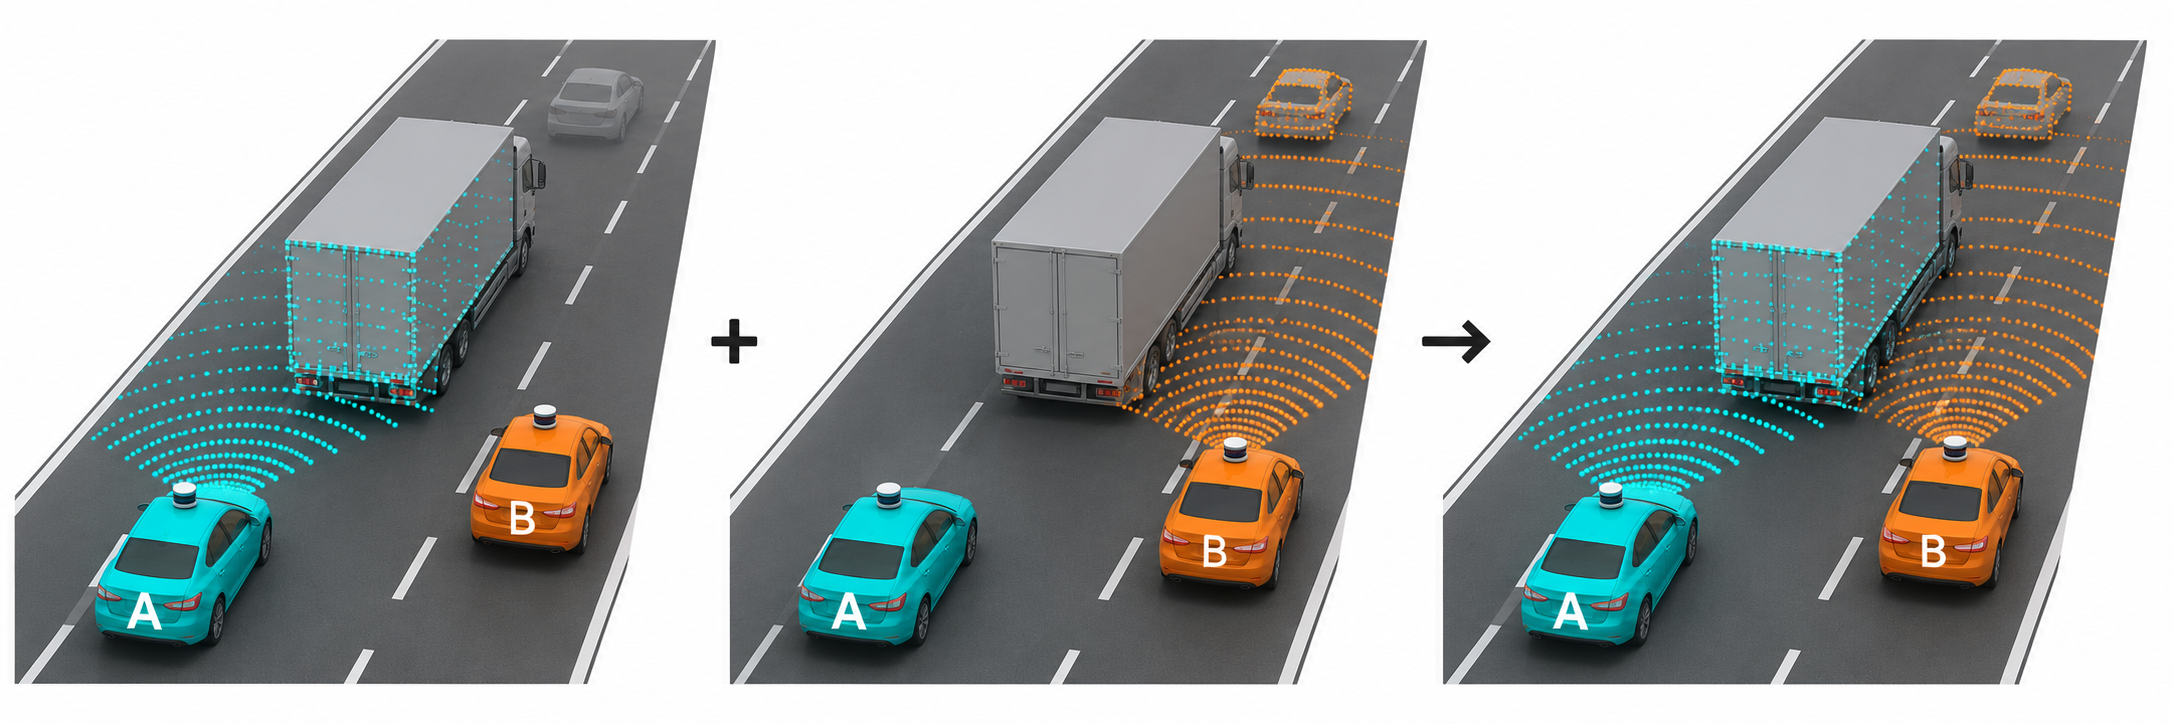
\includegraphics[width=14.65cm,height=4.90cm,keepaspectratio]
      {illustrations/prompt-trials-2026-11-09/layout-preservation-initial.png}\par
    \vspace{0.16cm}
    {\fontsize{11}{14}\selectfont Result from the prompt.\par}
  }
  \SlideSource{Source: AI generated illustration.}
\end{frame}

